\section{nonnative-inv}
\label{nonnative-inv}

\begin{enumerate}
    \item target
        check the multiplicatipn relation among three nonnative target objects.
    \item constraints-logic
        \begin{itemize}
            \item check equation for gadget,  a * inv-a = 1 + modular * div
        \end{itemize}
    \item nonnative-inv process layout
        \begin{figure}[!ht]
            \centering
            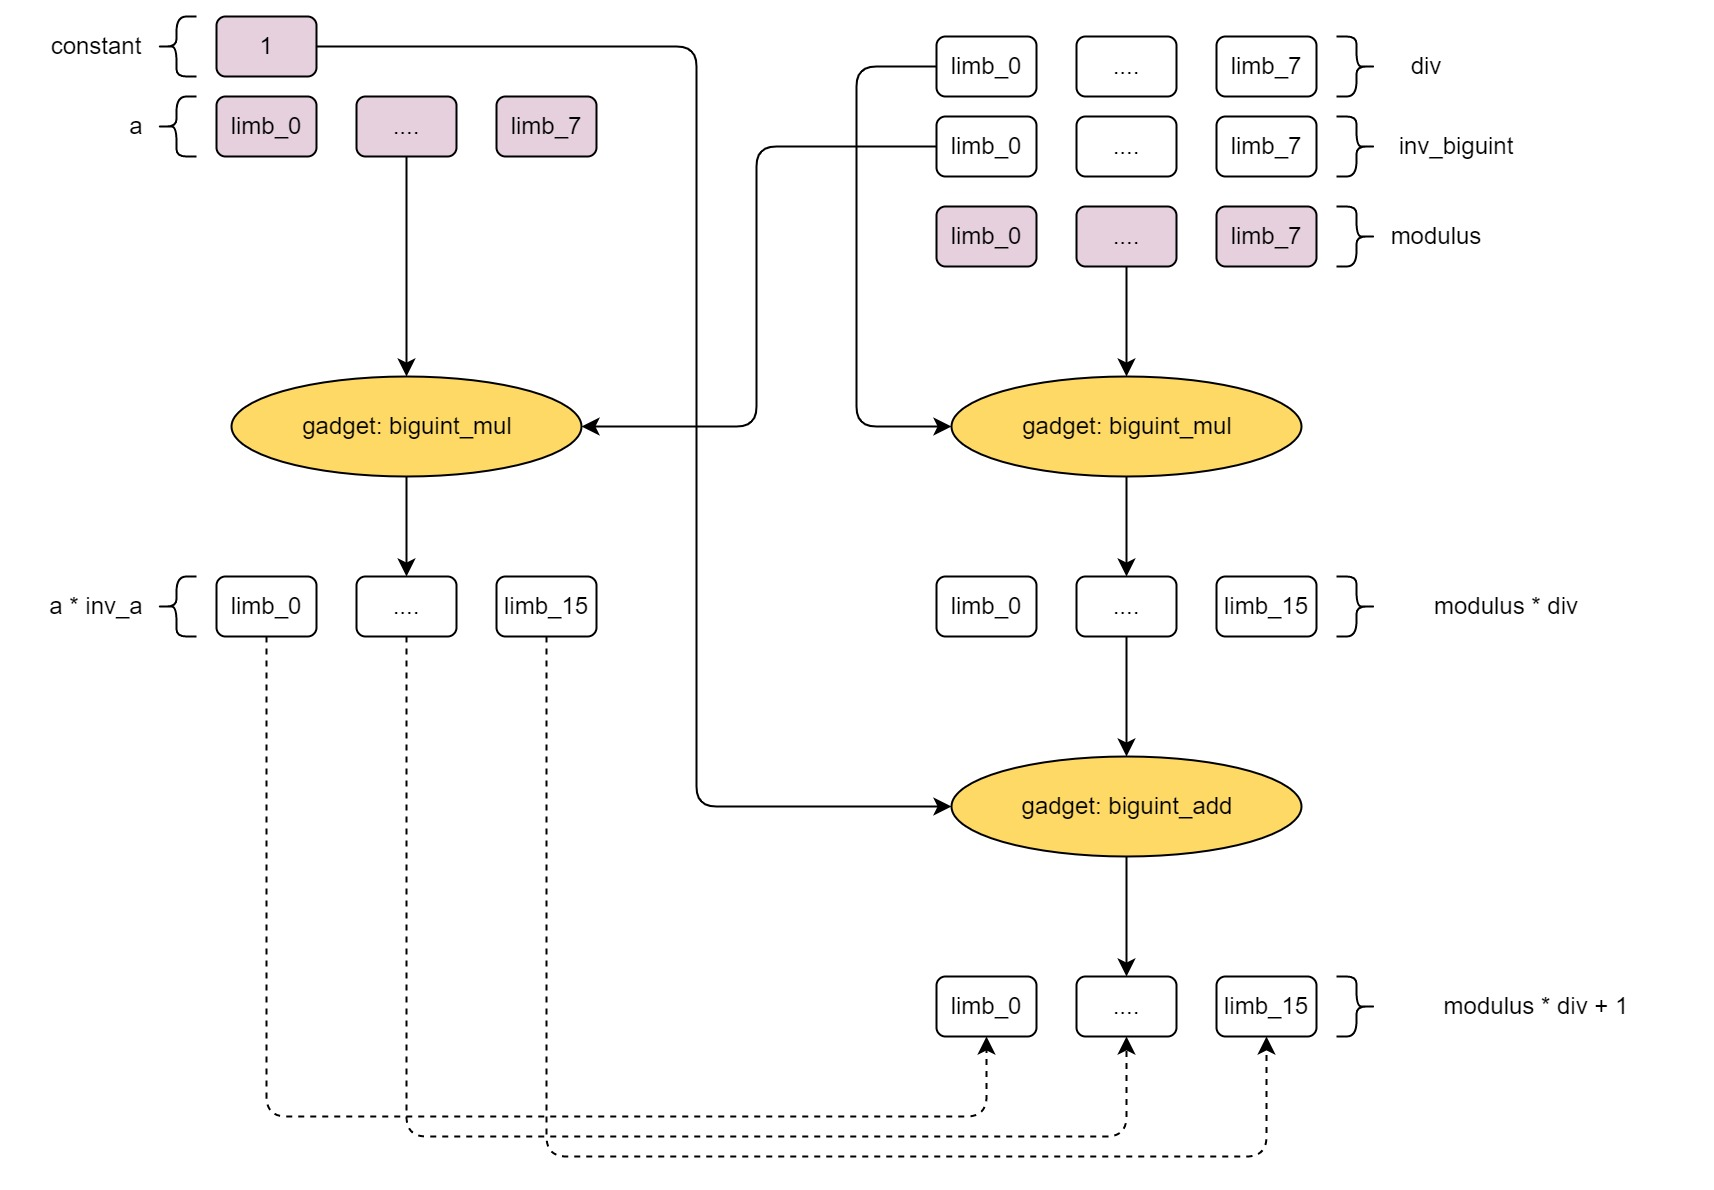
\includegraphics[width=0.8\textwidth]{nonnative-inv-layout.jpg}
            \caption{nonnative-inv layout}
            \label{fig:nonnative-inv-layout}
        \end{figure}
    
    \item constraints-info and costs
        \begin{itemize}
            \item gadget biguint-add num: 1
            \item gadget biguint-mul num: 2
            \item gate type num: 8 = 7(U32AddManyGate{3,5,7,9,11,13,15}) + 1(U32ArithmeticGate)
            \item gate instance num: 56 = (8 * 8 + 2) * 2 / 3 + 5(U32AddManyGate{3}) + 5 + 2(U32AddManyGate{15})
            \item copy-constraints: 762 = (8 * 8 + 2) * 2 * 3 + 21 * 4 + (6 + 8 + 10 + 12 + 14) * 4 + 4 * 16 + 18
        \end{itemize}

\end{enumerate}